\documentclass{standalone}
\usepackage{tikz}
\usetikzlibrary{patterns, positioning}
\usepackage[sfdefault]{ClearSans} %% option 'sfdefault' activates Clear Sans as the default text font
\usepackage[T1]{fontenc}

\begin{document}
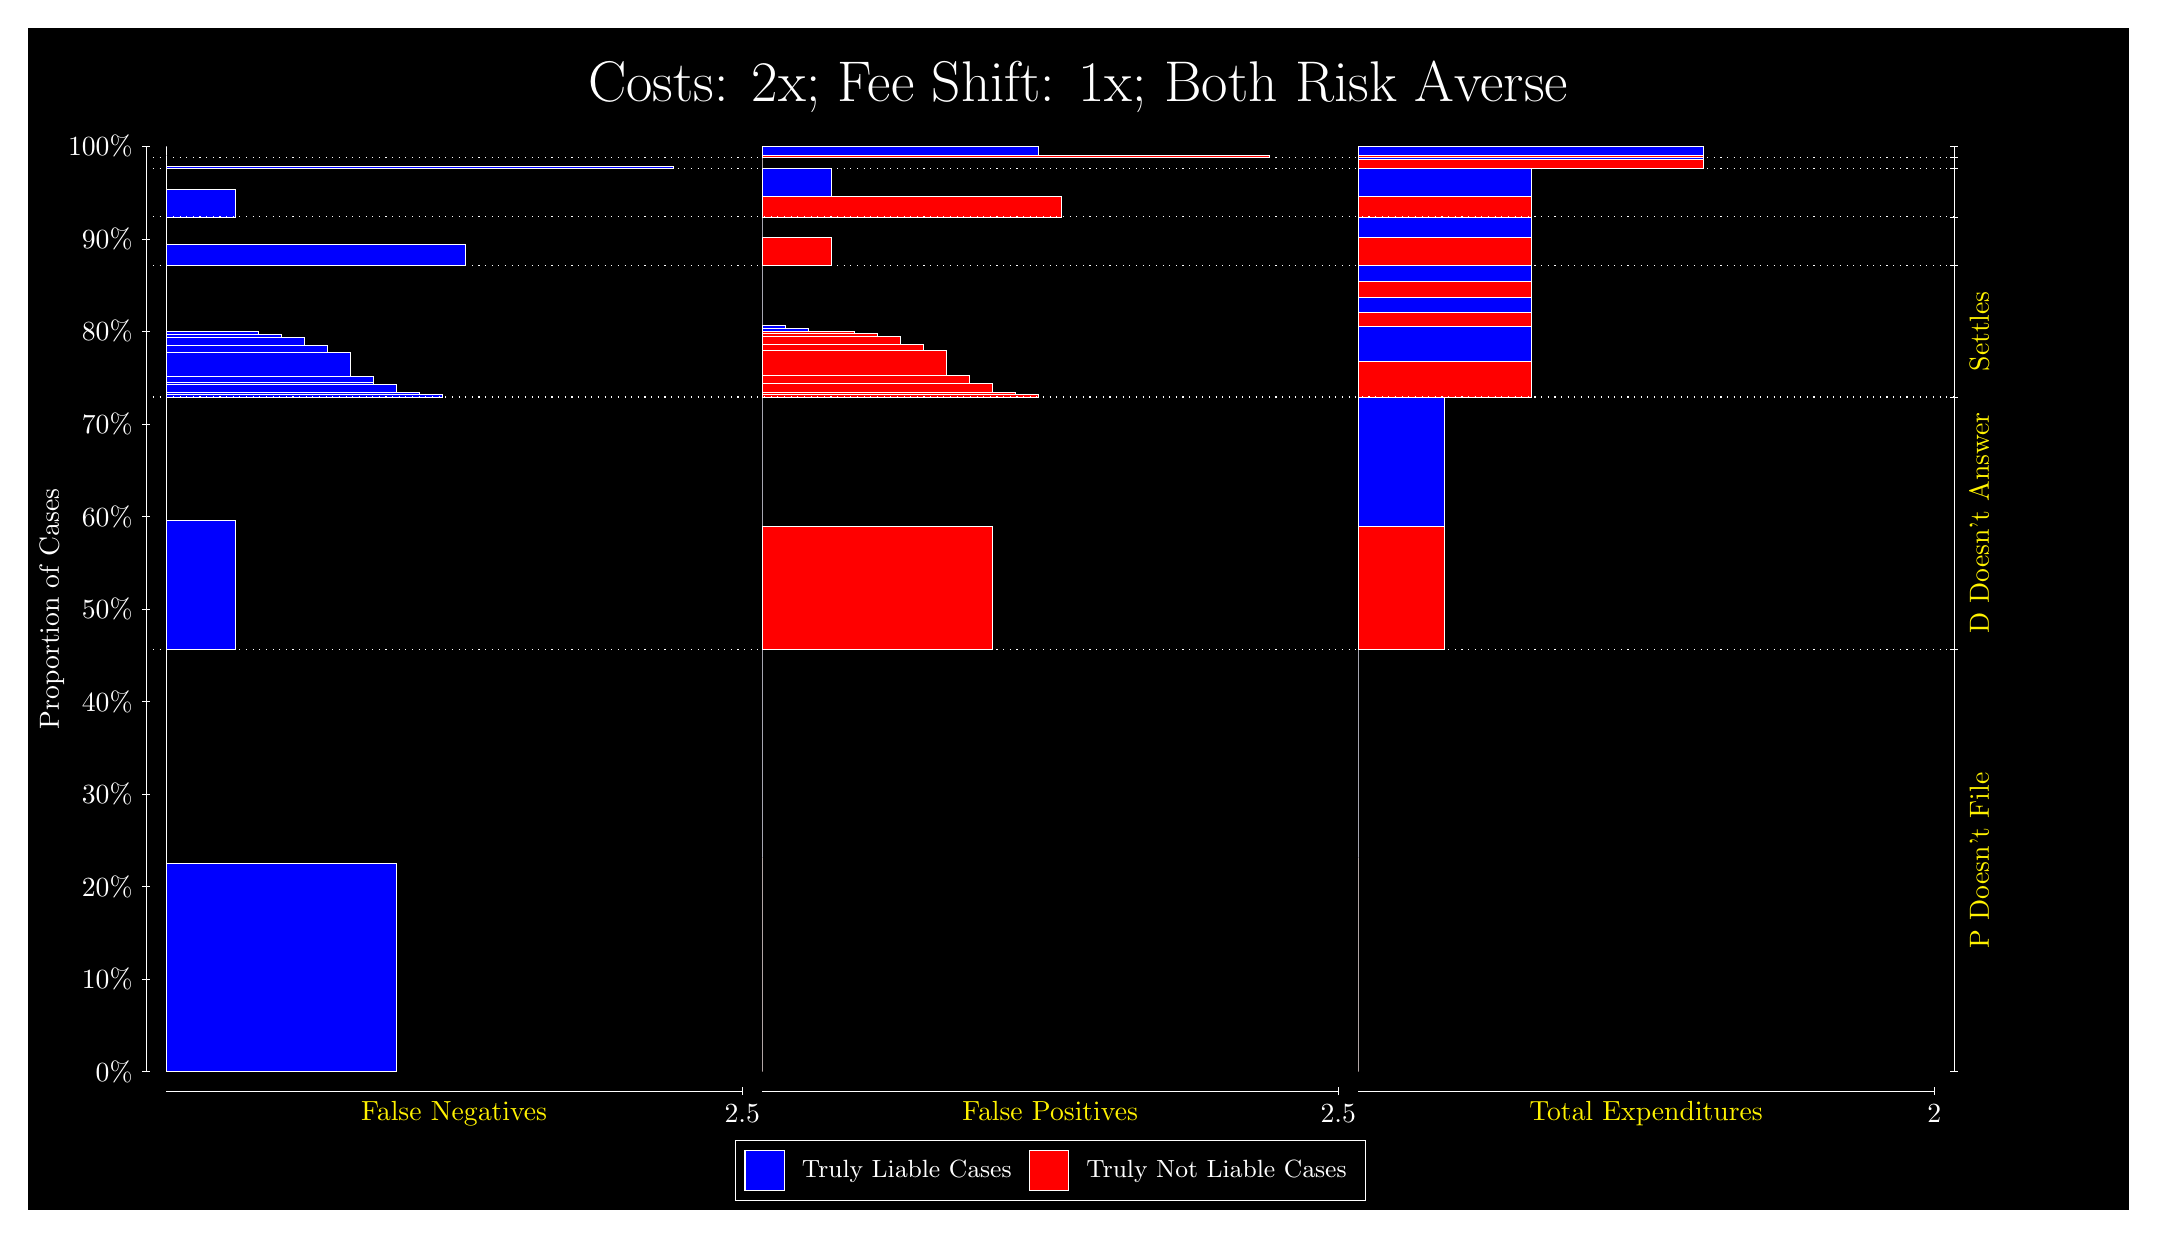
\begin{tikzpicture}
\draw[fill=black] (0,0) rectangle (26.667,15);
\draw[text=white] (0,13.5) rectangle (26.667,15) node[midway] {\huge Costs: 2x; Fee Shift: 1x; Both Risk Averse};
\draw[white, very thin] (1.5,1.75) -- (1.5,13.5);
\node[rotate=90, text=white, anchor=center] at (0.3, 7.625) {Proportion of Cases};
\draw[white, very thin] (1.45,1.75) -- (1.55,1.75);
\node[text=white, anchor=east] at (1.45, 1.75) {0\%};
\draw[white, very thin] (1.45,2.925) -- (1.55,2.925);
\node[text=white, anchor=east] at (1.45, 2.925) {10\%};
\draw[white, very thin] (1.45,4.1) -- (1.55,4.1);
\node[text=white, anchor=east] at (1.45, 4.1) {20\%};
\draw[white, very thin] (1.45,5.275) -- (1.55,5.275);
\node[text=white, anchor=east] at (1.45, 5.275) {30\%};
\draw[white, very thin] (1.45,6.45) -- (1.55,6.45);
\node[text=white, anchor=east] at (1.45, 6.45) {40\%};
\draw[white, very thin] (1.45,7.625) -- (1.55,7.625);
\node[text=white, anchor=east] at (1.45, 7.625) {50\%};
\draw[white, very thin] (1.45,8.8) -- (1.55,8.8);
\node[text=white, anchor=east] at (1.45, 8.8) {60\%};
\draw[white, very thin] (1.45,9.975) -- (1.55,9.975);
\node[text=white, anchor=east] at (1.45, 9.975) {70\%};
\draw[white, very thin] (1.45,11.15) -- (1.55,11.15);
\node[text=white, anchor=east] at (1.45, 11.15) {80\%};
\draw[white, very thin] (1.45,12.325) -- (1.55,12.325);
\node[text=white, anchor=east] at (1.45, 12.325) {90\%};
\draw[white, very thin] (1.45,13.5) -- (1.55,13.5);
\node[text=white, anchor=east] at (1.45, 13.5) {100\%};

\draw[white, very thin] (24.457,1.75) -- (24.457,13.5);
\draw[white, very thin] (24.407,1.75) -- (24.507,1.75);
\node[anchor=west] at (24.407, 1.75) {};
\draw[white, very thin] (24.407,7.1128) -- (24.507,7.1128);
\node[anchor=west] at (24.407, 7.1128) {};
\draw[white, very thin] (24.407,10.317) -- (24.507,10.317);
\node[anchor=west] at (24.407, 10.317) {};
\draw[white, very thin] (24.407,11.987) -- (24.507,11.987);
\node[anchor=west] at (24.407, 11.987) {};
\draw[white, very thin] (24.407,12.604) -- (24.507,12.604);
\node[anchor=west] at (24.407, 12.604) {};
\draw[white, very thin] (24.407,13.219) -- (24.507,13.219);
\node[anchor=west] at (24.407, 13.219) {};
\draw[white, very thin] (24.407,13.356) -- (24.507,13.356);
\node[anchor=west] at (24.407, 13.356) {};
\draw[white, very thin] (24.407,13.5) -- (24.507,13.5);
\node[anchor=west] at (24.407, 13.5) {};

\draw[white, very thin, fill=blue] (1.75,1.75) rectangle (4.6775,4.3972);
\draw[white, very thin, fill=red] (1.75,4.3972) rectangle (1.75,7.1128);
\draw[white, very thin, fill=blue] (1.75,7.1128) rectangle (2.6283,8.7523);
\draw[white, very thin, fill=red] (1.75,8.7523) rectangle (1.75,10.317);
\draw[white, very thin, fill=blue] (1.75,10.317) rectangle (5.2631,10.348);
\draw[white, very thin, fill=blue] (1.75,10.348) rectangle (4.9703,10.377);
\draw[white, very thin, fill=blue] (1.75,10.377) rectangle (4.6775,10.483);
\draw[white, very thin, fill=blue] (1.75,10.483) rectangle (4.3848,10.503);
\draw[white, very thin, fill=blue] (1.75,10.503) rectangle (4.3848,10.581);
\draw[white, very thin, fill=blue] (1.75,10.581) rectangle (4.092,10.888);
\draw[white, very thin, fill=blue] (1.75,10.888) rectangle (3.7993,10.978);
\draw[white, very thin, fill=blue] (1.75,10.978) rectangle (3.5065,11.08);
\draw[white, very thin, fill=blue] (1.75,11.08) rectangle (3.2138,11.114);
\draw[white, very thin, fill=blue] (1.75,11.114) rectangle (2.921,11.149);
\draw[white, very thin, fill=red] (1.75,11.149) rectangle (1.75,11.987);
\draw[white, very thin, fill=blue] (1.75,11.987) rectangle (5.5558,12.251);
\draw[white, very thin, fill=red] (1.75,12.251) rectangle (1.75,12.604);
\draw[white, very thin, fill=blue] (1.75,12.604) rectangle (2.6283,12.953);
\draw[white, very thin, fill=red] (1.75,12.953) rectangle (1.75,13.219);
\draw[white, very thin, fill=blue] (1.75,13.219) rectangle (8.1906,13.244);
\draw[white, very thin, fill=red] (1.75,13.244) rectangle (1.75,13.356);
\draw[white, very thin, fill=red] (1.75,13.356) rectangle (1.75,13.382);
\draw[white, very thin, fill=blue] (1.75,13.382) rectangle (1.75,13.5);
\draw[white, very thin, fill=red] (9.3189,1.75) rectangle (9.3189,4.4656);
\draw[white, very thin, fill=blue] (9.3189,4.4656) rectangle (9.3189,7.1128);
\draw[white, very thin, fill=red] (9.3189,7.1128) rectangle (12.246,8.6778);
\draw[white, very thin, fill=blue] (9.3189,8.6778) rectangle (9.3189,10.317);
\draw[white, very thin, fill=red] (9.3189,10.317) rectangle (12.832,10.348);
\draw[white, very thin, fill=red] (9.3189,10.348) rectangle (12.539,10.377);
\draw[white, very thin, fill=red] (9.3189,10.377) rectangle (12.246,10.491);
\draw[white, very thin, fill=red] (9.3189,10.491) rectangle (11.954,10.596);
\draw[white, very thin, fill=red] (9.3189,10.596) rectangle (11.661,10.906);
\draw[white, very thin, fill=red] (9.3189,10.906) rectangle (11.368,10.99);
\draw[white, very thin, fill=red] (9.3189,10.99) rectangle (11.075,11.087);
\draw[white, very thin, fill=red] (9.3189,11.087) rectangle (10.783,11.121);
\draw[white, very thin, fill=red] (9.3189,11.121) rectangle (10.49,11.155);
\draw[white, very thin, fill=blue] (9.3189,11.155) rectangle (9.9044,11.19);
\draw[white, very thin, fill=blue] (9.3189,11.19) rectangle (9.6116,11.224);
\draw[white, very thin, fill=blue] (9.3189,11.224) rectangle (9.3189,11.987);
\draw[white, very thin, fill=red] (9.3189,11.987) rectangle (10.197,12.34);
\draw[white, very thin, fill=blue] (9.3189,12.34) rectangle (9.3189,12.604);
\draw[white, very thin, fill=red] (9.3189,12.604) rectangle (13.125,12.869);
\draw[white, very thin, fill=blue] (9.3189,12.869) rectangle (10.197,13.219);
\draw[white, very thin, fill=red] (9.3189,13.219) rectangle (9.3189,13.33);
\draw[white, very thin, fill=blue] (9.3189,13.33) rectangle (9.3189,13.356);
\draw[white, very thin, fill=red] (9.3189,13.356) rectangle (15.759,13.382);
\draw[white, very thin, fill=blue] (9.3189,13.382) rectangle (12.832,13.5);
\draw[white, very thin, fill=red] (16.888,1.75) rectangle (16.888,4.4656);
\draw[white, very thin, fill=blue] (16.888,4.4656) rectangle (16.888,7.1128);
\draw[white, very thin, fill=red] (16.888,7.1128) rectangle (17.986,8.6778);
\draw[white, very thin, fill=blue] (16.888,8.6778) rectangle (17.986,10.317);
\draw[white, very thin, fill=red] (16.888,10.317) rectangle (19.083,10.769);
\draw[white, very thin, fill=blue] (16.888,10.769) rectangle (19.083,11.213);
\draw[white, very thin, fill=red] (16.888,11.213) rectangle (19.083,11.398);
\draw[white, very thin, fill=blue] (16.888,11.398) rectangle (19.083,11.584);
\draw[white, very thin, fill=red] (16.888,11.584) rectangle (19.083,11.785);
\draw[white, very thin, fill=blue] (16.888,11.785) rectangle (19.083,11.987);
\draw[white, very thin, fill=red] (16.888,11.987) rectangle (19.083,12.34);
\draw[white, very thin, fill=blue] (16.888,12.34) rectangle (19.083,12.604);
\draw[white, very thin, fill=red] (16.888,12.604) rectangle (19.083,12.869);
\draw[white, very thin, fill=blue] (16.888,12.869) rectangle (19.083,13.219);
\draw[white, very thin, fill=red] (16.888,13.219) rectangle (21.279,13.33);
\draw[white, very thin, fill=blue] (16.888,13.33) rectangle (21.279,13.356);
\draw[white, very thin, fill=red] (16.888,13.356) rectangle (21.279,13.382);
\draw[white, very thin, fill=blue] (16.888,13.382) rectangle (21.279,13.5);
\draw[white, dotted] (1.5,7.1128) -- (24.457,7.1128);
\draw[white, dotted] (1.5,10.317) -- (24.457,10.317);
\draw[white, dotted] (1.5,11.987) -- (24.457,11.987);
\draw[white, dotted] (1.5,12.604) -- (24.457,12.604);
\draw[white, dotted] (1.5,13.219) -- (24.457,13.219);
\draw[white, dotted] (1.5,13.356) -- (24.457,13.356);
\draw[white, very thin] (1.75,1.5) -- (9.0689,1.5);
\node[text=yellow, anchor=north] at (5.4094, 1.5) {False Negatives};
\draw[white, very thin] (9.0689,1.45) -- (9.0689,1.55);
\node[text=white, anchor=north] at (9.0689, 1.45) {2.5};

\draw[white, very thin] (9.3189,1.5) -- (16.638,1.5);
\node[text=yellow, anchor=north] at (12.978, 1.5) {False Positives};
\draw[white, very thin] (16.638,1.45) -- (16.638,1.55);
\node[text=white, anchor=north] at (16.638, 1.45) {2.5};

\draw[white, very thin] (16.888,1.5) -- (24.207,1.5);
\node[text=yellow, anchor=north] at (20.547, 1.5) {Total Expenditures};
\draw[white, very thin] (24.207,1.45) -- (24.207,1.55);
\node[text=white, anchor=north] at (24.207, 1.45) {2};

\node[text=yellow, centered, rotate=90] at (24.777, 4.4314) {P Doesn't File};
\node[text=yellow, centered, rotate=90] at (24.777, 8.7151) {D Doesn't Answer};
\node[text=yellow, centered, rotate=90] at (24.777, 11.152) {Settles};





\draw (12.978300999999998,1.5) node[draw=none] (baseCoordinate) {};
\begin{scope}[align=center]
        \matrix[scale=0.5, draw=white, below=0.5cm of baseCoordinate, nodes={draw}, column sep=0.1cm]{
            \node[rectangle, draw, minimum width=0.5cm, minimum height=0.5cm, fill=blue] {}; &
            \node[draw=none, font=\small, text=white] (B) {Truly Liable Cases}; &
            \node[rectangle, draw, minimum width=0.5cm, minimum height=0.5cm, fill=red] {}; &
            \node[draw=none, font=\small, text=white] (B) {Truly Not Liable Cases}; \\
            };
\end{scope}

\end{tikzpicture}
\end{document}